%%%%%%%%%%%%%%%%%%%%%%%%%%%%%%%%%%%%%%%%%%%%%%%%%%%%%%%%%%%%%%%%%%%
%TO AVOID FORMATTING ISSUES, COMPILE THIS ONLY AT WWW.OVERLEAF.COM%
%%%%%%%%%%%%%%%%%%%%%%%%%%%%%%%%%%%%%%%%%%%%%%%%%%%%%%%%%%%%%%%%%%%
%%%%%%%%%%%%%%%%%%%%%%%%%%%%%%%%%%%%%%%%%%%%%%%%%%%%%%%%%%%%%%%%%%%
\documentclass[a4paper,12pt]{article}
\usepackage{graphicx}
%To use this font, you need XeTex or LuaTex, prefer openleaf
\newenvironment{codeblock}{\fontfamily{ccr}\selectfont}{\par}

\title{
	\normalfont \normalsize 
	\textsc{Pimpri Chinchwad College of Engineering \\ 
		Computer Laboratory - IV} \\
	[10pt]   
	\rule{\linewidth}{0.5pt} \\[6pt] 
	\huge Assignment No - B2 \\
	\rule{\linewidth}{2pt}  \\[10pt]
}
\author{}
\date{\normalsize}


\begin{document}
	\maketitle

\textbf{AIM: } A Web application for Concurrent implementation of ODD-EVEN SORT is to be designed using Real time Object Oriented Modeling(ROOM). Give the necessary design diagrams and write the test cases for the white box testing. Draw Concurrent collaboration Diagrams.
\\

\noindent \textbf{OBJECTIVE:}
\begin{itemize}
\item To implement the Odd-Even Sort algorithm using C++.
\item To test the resultant application using White-box testing techniques.
\end{itemize}
\noindent \textbf{UML diagrams :}\\
\begin{itemize}
\item \textbf{Class diagram :}
\begin{figure}[h!]
		\centering
		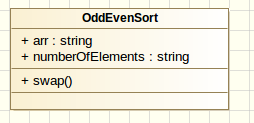
\includegraphics[scale=0.5]{oddEven.png}
	\end{figure}
\item \textbf{Collaboration Diagram :}\\
\begin{figure}[h!]
		\centering
		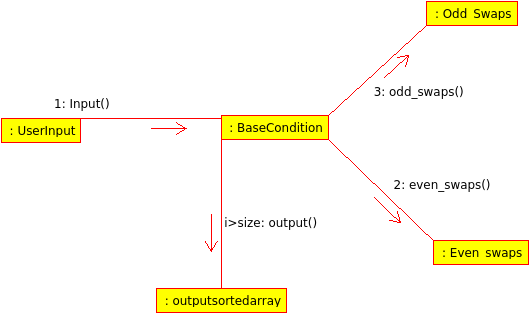
\includegraphics[scale=0.5]{oddevencoll.png}
	\end{figure}
\newpage
\item \textbf{Flowchart :}\\
\bigskip

\begin{figure}[h!]
		\centering
		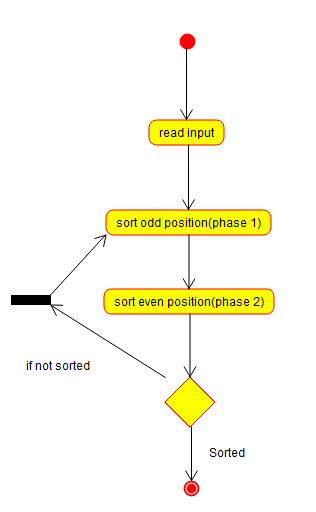
\includegraphics[scale=0.5]{odd-even-activity}
	\end{figure}




\bigskip
\bigskip

\end{itemize}

\bigskip
\bigskip
\noindent \textbf{MATHEMATICAL MODEL:}\\[0.5cm]
S=\{s,e,X,Y,Fme,DD,NDD\}\\[0.5cm]

\textbf{s=Initial State}\\
The program does not contain any previously initialized values
\\[0.5cm]
\textbf{e=End State}\\

Sorting is performed using the mentioned algorithm, which is Odd-even sort. After passing the values to the program, the appropriate function calculates the output values which are in sorted order.
\\

\textbf{X=Input given}\\
The input given to the app are random numbers which are to be sorted.
\\

\textbf{Y=Output obtained}\\
  The output of the app is the resultant sorted array after sorting operations using the Odd-Even sort.
 \\

\textbf{Fme=Function/Algorithm}\\
The algorithm consists of functions various condition statements which check whether the give index of the array is even, or odd. Appropriate swapping takes place in either of the cases. 
\\

\textbf{DD=Deterministic data}\\
There is no deterministic data in the application.
\\

\textbf{NDD=Non-deterministic data}\\
The output will be dependent upon what input the user provides. 
\\

\noindent \textbf{Theory:}\\
\begin{itemize}
\item \textbf{Servlet:}
Servlet can be described in many ways, depending on the context.
\begin{itemize}
\item Servlet is a technology i.e. used to create web application.
\item Servlet is an API that provides many interfaces and classes including documentations.
\item Servlet is an interface that must be implemented for creating any servlet.
\item Servlet is a class that extend the capabilities of the servers and respond to the incoming request. It can respond to any type of requests.
\item Servlet is a web component that is deployed on the server to create dynamic web page.
\begin{figure}[h!]
		\centering
		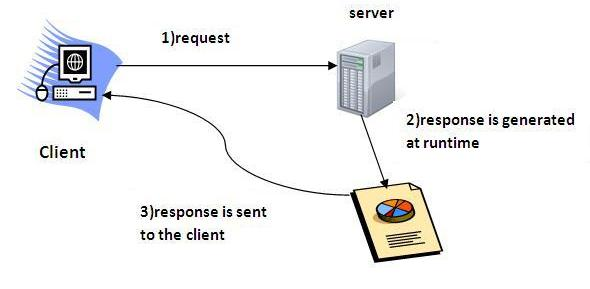
\includegraphics[scale=0.5]{response.JPG}
	\end{figure}
\end{itemize}
A Java servlet is a Java program that extends the capabilities of a server. Although servlets can respond to any types of requests, they most commonly implement applications hosted on Web servers.
\end{itemize}

\begin{itemize}
\item \textbf{Odd-Even sort:}
An odd–even sort or odd–even transposition sort (also known as brick sort) is a relatively simple sorting algorithm, developed originally for use on parallel processors with local interconnections. It is a comparison sort related to bubble sort, with which it shares many characteristics. It functions by comparing all odd/even indexed pairs of adjacent elements in the list and, if a pair is in the wrong order (the first is larger than the second) the elements are switched. The next step repeats this for even/odd indexed pairs (of adjacent elements). Then it alternates between odd/even and even/odd steps until the list is sorted.
\end{itemize}

\begin{itemize}
\item \textbf{Sorting on processor arrays:}\\
On parallel processors, with one value per processor and only local left–right neighbor connections, the processors all concurrently do a compare–exchange operation with their neighbors, alternating between odd–even and even–odd pairings.
\end{itemize}

\noindent \textbf{Testing:}
\begin{itemize}
\item \textbf{White-box testing:}\\
White-box testing (also known as clear box testing, glass box testing, transparent box testing, and structural testing) is a method of testing software that tests internal structures or workings of an application, as opposed to its functionality (i.e. black-box testing). 

In white-box testing an internal perspective of the system, as well as programming skills, are used to design test cases. The tester chooses inputs to exercise paths through the code and determine the appropriate outputs. This is analogous to testing nodes in a circuit, e.g. in-circuit testing (ICT). White-box testing can be applied at the unit, integration and system levels of the software testing process.

White-box test design techniques include the following code coverage criteria:

    
\begin{itemize}
\item Control flow testing
\end{itemize}
\begin{itemize}
\item Data flow testing
\end{itemize}
\begin{itemize}
\item Branch testing
\end{itemize}
\begin{itemize}
\item Statement coverage
\end{itemize}
\begin{itemize}
\item Decision coverage
\end{itemize}
\begin{itemize}
\item Modified condition/decision coverage
\end{itemize}
\begin{itemize}
\item Prime path testing
\end{itemize}
\begin{itemize}
\item Path testing

\end{itemize}
\end{itemize}
\bigskip
\begin{itemize}
\item \textbf{Test cases using white box testing :}
\begin{figure}[h!]
		\centering
		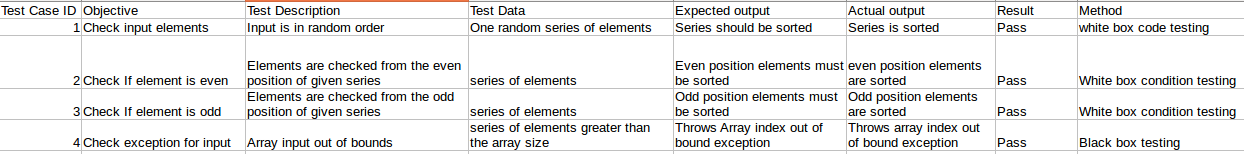
\includegraphics[width=\textwidth]{testcase.png}
	\end{figure}


\bigskip
\bigskip

\end{itemize}
\noindent \textbf{White box testing:}\\[0.5cm]
\begin{enumerate}
  \item No of Loops : 3
  \item No of Conditions : 10
  \item No of Plain Statements :6
  \item Total Lines : 65
\end{enumerate}

Enter the number of elements
5

Hence size = 5

Enter the elements
8 1 4 3 9

\bigskip
\bigskip

Testing Loops for Sorting\par
Looping Variables i,j,k\par
k - Outer For Loop\par
i - Inner k%2==0 True Condition For Loop\par
j - Inner k%2==0 False Condition For Loop\par

Initially k = 0\\\par


Iteration No 1\par
k=0\par
k\%2==0 is True Hence Swap Even Positions\par
if(i!=arr.length-1) is True\par
if(arr[i]\textgreater arr[i+1]) is True in case of{(a[0],a[1]),(a[2],a[3])}\par
Inner Loop Ends Successfully when i \textgreater size\par
1 8 3 4 9\\\par


Iteration No 2\par
k=1\par
k\%2==0 is False Hence Swap Odd Positions\par
if(i!=arr.length-1) is True\par
if(arr[i] \textgreater arr[i+1]) is True in case of{(a[1],a[2])}\par
Inner Loop Ends Successfully when j \textgreater size\par
1 3 8 4 9\\\par


Iteration No 3\par
k=2\par
k\%2==0 is True Hence Swap Even Positions\par
if(i!=arr.length-1) is True\par
if(arr[i] \textgreater arr[i+1]) is True in case of{(a[2],a[3])}\par
Inner Loop Ends Successfully when i \textgreater size\par
1 3 4 8 9\\\par


Iteration No 4\par
k=3\par
k\%2==0 is False Hence Swap Odd Positions\par
if(i!=arr.length-1) is True\par  
if(arr[i] \textgreater arr[i+1]) is False In case of All\par
Inner Loop Ends Successfully when j \textgreater size\par
1 3 4 8 9\\\par


Iteration No 5\par
k=4\par
k\%2==0 is True Hence Swap Even Positions\par
if(i!=arr.length-1) is True\par
if(arr[i] \textgreater arr[i+1]) is False In case of All\par
Inner Loop Ends Successfully when i \textgreater size\par
1 3 4 8 9\\\par

Iteration 6\par
k=5\par
k<size is False Hence Sorting Loops are completely executed.\par
Tested Completely\\\par


Thus All Paths Are Tested Successfully and Code Coverage is 100\% as each line is executed atleast once.\\\par

\begin{itemize}
\item \textbf{Real-Time Object-Oriented Modeling (ROOM)}
Model real time systems based on timeliness, dynamic internal structure, reactiveness, concurrency and distribution, using the ROOM notation.\\
\textbf{ROOM} is an object-oriented methodology for real-time systems developed originally at Bell-Northern Research. ROOM is based upon a principle of using the same model for all phases of the development process. ROOM models are composed of actors which communicate with each other by sending messages along protocols. Actors may be hierarchically decomposed, and may have behaviors described by ROOM charts, a variant of Harel's state charts. Descriptions of actors, protocols, and behaviors can all be reused through inheritance.
\end{itemize}

\begin{itemize}
	\item\textbf{ROOM Diagram Software Features}
	
	\item Chart Templates
	
	
	
	\item Symbol Gallery
	
	\item Drag and Drop Interface
	
	
	
	\item Grids \& Guides
	
	\item Snap-to
	
	
	
	\item Change Existing Diagram Shapes
	
	\item Automatic Spacing \& Alignment
	
	
	
	\item Multiple Connector Points
	
	\item Change Connector Path
	
	
	
	\item Connector Labels
	
	\item Add Connector Points to Symbols
	
	
	
	\item Junction Jogs
	
	\item Multiple Pages
	
	
	
	\item Add Hyperlinks
	
	\item Grouping Shapes
	
	
	
	\item Expandable Canvas
	
\end{itemize}

\noindent \textbf{Conclusion: }	\\
We have studied and implemented an Odd-Even sort algorithm in C++, and applied White-box testing techniques.

\begin{center}
\begin{tabular}
{|c|c|c|c|c|}\hline
{\bf Roll No.}		&{\bf Name of Student}	&{\bf Date of Performance}  				&{\bf Date of Submission}	&{\bf Sign.}  \\    \hline
{302}	&	{Abhinav Bakshi}& 	{29/02/16}	&  {21/03/16} \\ \hline
\end{tabular}\\ 
\end{center}


\begin{figure}[htb!]
	\centering
	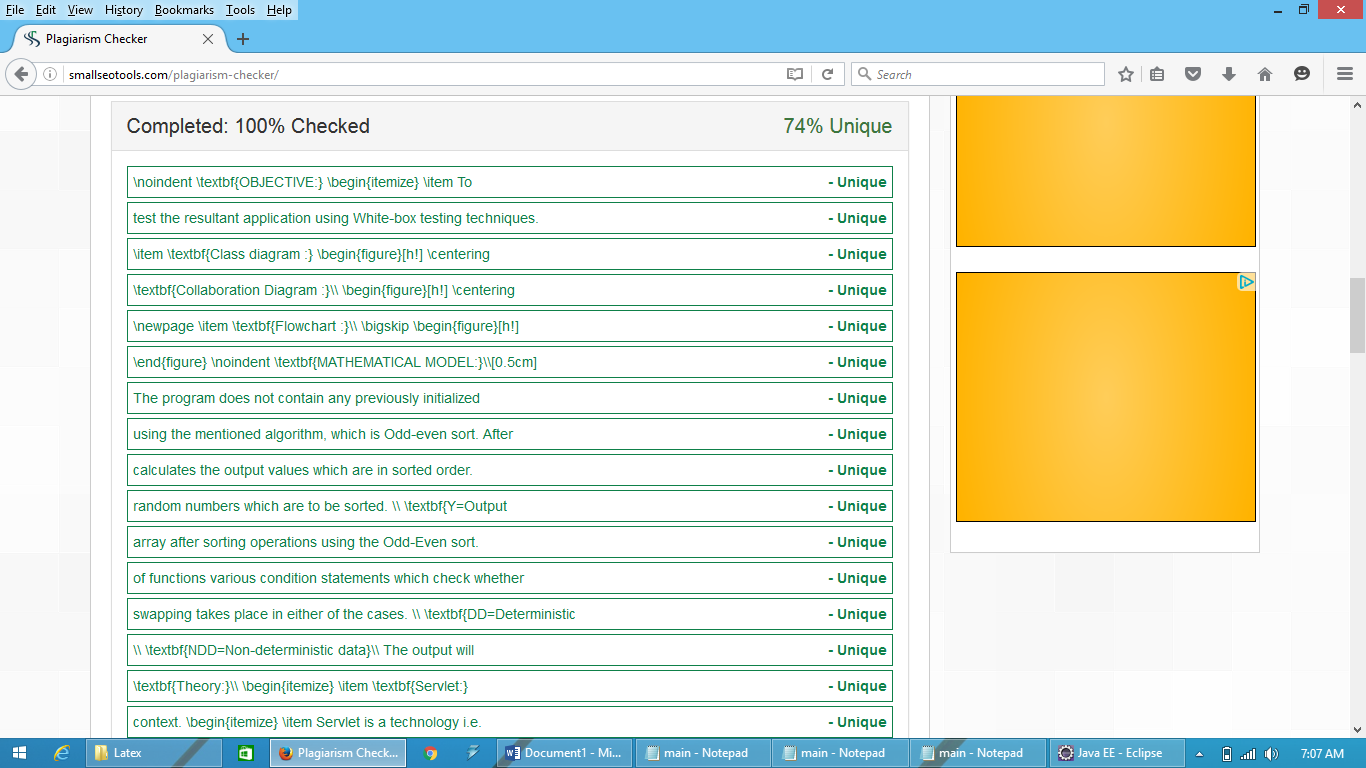
\includegraphics[scale = 0.80]{b2_oddeven.png}
	\caption{Plagiarism Report }
	\label{Plagiarism Report}
\end{figure}



\end{document}



 
